\documentclass{article}
\usepackage[margin=1in]{geometry}
\usepackage[utf8]{inputenc}
\usepackage{amsmath}
\usepackage{tikz}
\usepackage{pgfplots}
\usepackage{color}
\usepackage{amsfonts}
\usepackage{amssymb}
\usepackage{graphicx}

\title{Homework 2}
\author{Giacomo Cappelletto}
\date{\today}

\begin{document}

\maketitle

\section*{Problem 1 - Section A}

\subsection*{System 1}

\subsubsection*{A}
\begin{figure}[h!]
	\centering
	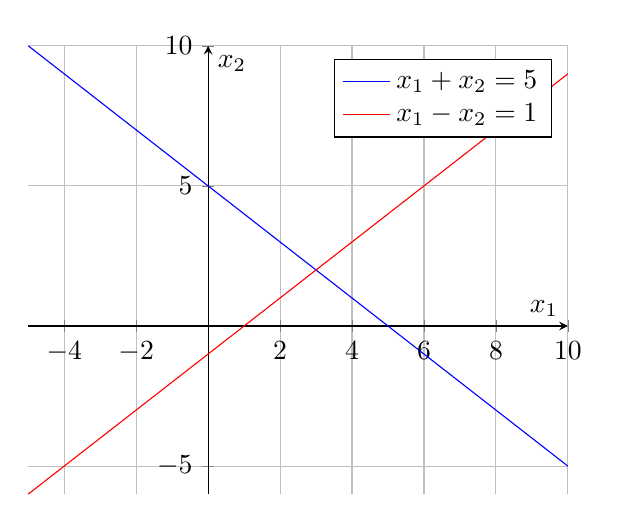
\begin{tikzpicture}
		\begin{axis}[
				axis lines = middle,
				xlabel = $x_1$,
				ylabel = $x_2$,
				grid = both,
				legend pos = north east
			]
			% Plot of x + y = 5
			\addplot[
				domain=-5:10,
				samples=20,
				color=blue
			]
			{5 - x};
			\addlegendentry{$x_1 + x_2 = 5$}

			% Plot of x - y = 1
			\addplot[
				domain=-5:10,
				samples=20,
				color=red
			]
			{x - 1};
			\addlegendentry{$x_1 - x_2 = 1$}


		\end{axis}
	\end{tikzpicture}
	\caption{Plot of $x_1 + x_2 = 5$ and $x_1 - x_2 = 1$}
	\label{fig:plot1}
\end{figure}

\subsubsection*{B}

A unique solution since there is one intersection point between the lines.

\subsubsection*{C}

\[
	\begin{bmatrix}
		1 & 1  \\
		1 & -1
	\end{bmatrix}
	\cdot
	\begin{bmatrix}
		x_1 \\
		x_2
	\end{bmatrix}
	=
	\begin{bmatrix}
		5 \\
		1
	\end{bmatrix}
\]

\subsubsection*{D}

\[
	\begin{bmatrix}
		1 & 1  & 5 \\
		1 & -1 & 1
	\end{bmatrix}
\]

\subsubsection*{E}

\[
	\begin{bmatrix}
		1 & 1  & 5 \\
		1 & -1 & 1
	\end{bmatrix}
	\xrightarrow{R_2 = R_2 - R_1}
	\begin{bmatrix}
		1 & 1  & 5  \\
		0 & -2 & -4
	\end{bmatrix}
\]

\subsubsection*{F}

\[
	\begin{bmatrix}
		1 & 1  & 5  \\
		0 & -2 & -4
	\end{bmatrix}
	\xrightarrow{R_2 = -\frac{1}{2}R_2}
	\begin{bmatrix}
		1 & 1 & 5 \\
		0 & 1 & 2
	\end{bmatrix}
	\xrightarrow{R_1 = R_1 - R_2}
	\begin{bmatrix}
		1 & 0 & 3 \\
		0 & 1 & 2
	\end{bmatrix}
\]

Therefore, given this RREF, it follows that

\[
	\begin{bmatrix}
		x_1 \\
		x_2
	\end{bmatrix}
	=
	\begin{bmatrix}
		3 \\
		2
	\end{bmatrix}
\]

\subsection*{System 2}

\subsubsection*{A}

\begin{figure}[h!]
	\centering
	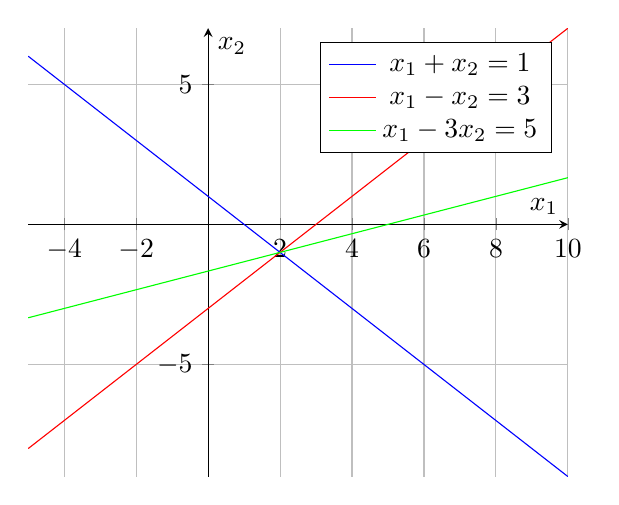
\begin{tikzpicture}
		\begin{axis}[
				axis lines = middle,
				xlabel = $x_1$,
				ylabel = $x_2$,
				grid = both,
				legend pos = north east
			]
			% Plot of x + y = 5
			\addplot[
				domain=-5:10,
				samples=20,
				color=blue
			]
			{1 - x};
			\addlegendentry{$x_1 + x_2 = 1$}

			% Plot of x - y = 1
			\addplot[
				domain=-5:10,
				samples=20,
				color=red
			]
			{x - 3};
			\addlegendentry{$x_1 - x_2 = 3$}

			% Plot of x - y = 1
			\addplot[
				domain=-5:10,
				samples=20,
				color=green
			]
			{(x/3) - (5/3)};
			\addlegendentry{$x_1 - 3x_2 = 5$}


		\end{axis}
	\end{tikzpicture}
	\caption{Plot of $x_1 + x_2 = 1$, $x_1 - x_2 = 3$, and $x_1 - 3x_2 = 5$}
	\label{fig:plot2}
\end{figure}

\subsubsection*{B}

The SLE will have one solution since all lines intersect at the same point.

\subsubsection*{C}

\[
	\begin{bmatrix}
		1 & 1  \\
		1 & -1 \\
		1 & -3
	\end{bmatrix}
	\cdot
	\begin{bmatrix}
		x_1 \\
		x_2
	\end{bmatrix}
	=
	\begin{bmatrix}
		1 \\
		3 \\
		5
	\end{bmatrix}
\]

\subsubsection*{D}

\[
	\begin{bmatrix}
		1 & 1  & 1 \\
		1 & -1 & 3 \\
		1 & -3 & 5
	\end{bmatrix}
\]

\subsubsection*{E}

\[
	\begin{bmatrix}
		1 & 1  & 1 \\
		1 & -1 & 3 \\
		1 & -3 & 5
	\end{bmatrix}
	\xrightarrow{R_2 = R_2 - R_1, R_3 = R_3 - R_1}
	\begin{bmatrix}
		1 & 1  & 1 \\
		0 & -2 & 2 \\
		0 & -4 & 4
	\end{bmatrix}
	\xrightarrow{R_3 = R_3 - 2R_2}
	\begin{bmatrix}
		1 & 1  & 1 \\
		0 & -2 & 2 \\
		0 & 0  & 0
	\end{bmatrix}
\]

\[
	\begin{bmatrix}
		1 & 1  & 1 \\
		0 & -2 & 2 \\
		0 & 0  & 0
	\end{bmatrix}
	\xrightarrow{R_2 = -\frac{1}{2}R_2}
	\begin{bmatrix}
		1 & 1 & 1  \\
		0 & 1 & -1 \\
		0 & 0 & 0
	\end{bmatrix}
	\xrightarrow{R_1 = R_1 - R_2}
	\begin{bmatrix}
		1 & 0 & 2  \\
		0 & 1 & -1 \\
		0 & 0 & 0
	\end{bmatrix}
\]
Therefore, given this RREF, it follows that

\[
	\begin{bmatrix}
		x_1 \\
		x_2
	\end{bmatrix}
	=
	\begin{bmatrix}
		2 \\
		-1
	\end{bmatrix}
\]

\subsection*{System 3}

\subsubsection*{A}

\begin{figure}[h!]
	\centering
	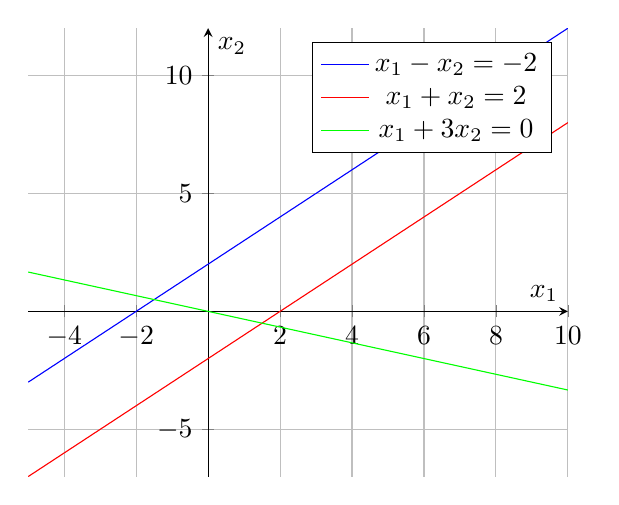
\begin{tikzpicture}
		\begin{axis}[
				axis lines = middle,
				xlabel = $x_1$,
				ylabel = $x_2$,
				grid = both,
				legend pos = north east
			]
			\addplot[
				domain=-5:10,
				samples=20,
				color=blue
			]
			{x+2};
			\addlegendentry{$x_1 - x_2 = -2$}

			\addplot[
				domain=-5:10,
				samples=20,
				color=red
			]
			{x - 2};
			\addlegendentry{$x_1 + x_2 = 2$}

			\addplot[
				domain=-5:10,
				samples=20,
				color=green
			]
			{-x/3};
			\addlegendentry{$x_1 + 3x_2 = 0$}

		\end{axis}
	\end{tikzpicture}
	\caption{Plot of $x_1 - x_2 = -2$, $x_1 + x_2 = 2$, and $x_1 + 3x_2 = 0$}
	\label{fig:plot3}
\end{figure}

\subsubsection*{B}

No solution to SLE since the lines do not all have common intersection point.

\subsubsection*{C}

\[
	\begin{bmatrix}
		1 & 1 \\
		1 & 1 \\
		1 & 3
	\end{bmatrix}
	\cdot
	\begin{bmatrix}
		x_1 \\
		x_2
	\end{bmatrix}
	=
	\begin{bmatrix}
		-2 \\
		2  \\
		0
	\end{bmatrix}
\]

\subsubsection*{D}

\[
	\begin{bmatrix}
		1 & -1 & -2 \\
		1 & 1  & 2  \\
		1 & 3  & 0
	\end{bmatrix}
\]

\subsubsection*{E}

\[
	\begin{bmatrix}
		1 & -1 & -2 \\
		1 & 1  & 2  \\
		1 & 3  & 0
	\end{bmatrix}
	\xrightarrow{R_2 = R_2 - R_1 ,R_3 = R_3 - R_1}
	\begin{bmatrix}
		1 & -1 & 2 \\
		0 & 2  & 4 \\
		0 & 4  & 2
	\end{bmatrix}
	\xrightarrow{R_3 = R_3 - 2R_2}
	\begin{bmatrix}
		1 & -1 & 2  \\
		0 & 2  & 4  \\
		0 & 0  & -6
	\end{bmatrix}
\]

\subsubsection*{F}

The last column of the REF effectively shows that $x_1 \cdot 0 = -6$, which is sufficient to determine that the SLE is not consistent.

\section*{Problem 1 - Section B}

\subsection*{System 4}

\begin{figure}[h!]
	\centering
	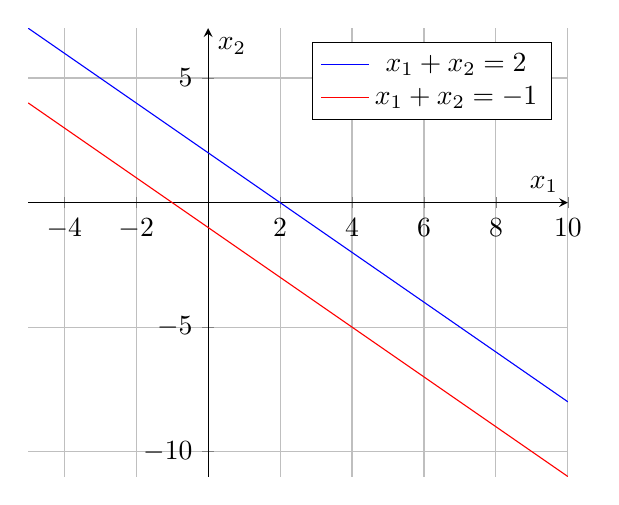
\begin{tikzpicture}
		\begin{axis}[
				axis lines = middle,
				xlabel = $x_1$,
				ylabel = $x_2$,
				grid = both,
				legend pos = north east
			]
			% Plot of x + y = 5
			\addplot[
				domain=-5:10,
				samples=20,
				color=blue
			]
			{2 - x};
			\addlegendentry{$x_1 + x_2 = 2$}

			% Plot of x - y = 1
			\addplot[
				domain=-5:10,
				samples=20,
				color=red
			]
			{-x - 1};
			\addlegendentry{$x_1 + x_2 = -1$}


		\end{axis}
	\end{tikzpicture}
	\caption{Plot of $x_1 + x_2 = 2$ and $x_1 + x_2 = -1$}
	\label{fig:plot4}
\end{figure}

\subsubsection*{B}

The SLE will have no solutions since the lines are parallel and therefore will never intersect.

\subsubsection*{C}

\[
	\begin{bmatrix}
		1 & 1 & 2  \\
		1 & 1 & -2
	\end{bmatrix}
	\xrightarrow{R_2 = R_2 - R_1}
	\begin{bmatrix}
		1 & 1 & 2 \\
		0 & 0 & 4
	\end{bmatrix}
	\xrightarrow{R_2 = -\frac{1}{4}R_2}
	\begin{bmatrix}
		1 & 1 & 2 \\
		0 & 0 & 1
	\end{bmatrix}
	\xrightarrow{R_1 = R_1 - 2R_2}
	\begin{bmatrix}
		1 & 1 & 0 \\
		0 & 0 & 1
	\end{bmatrix}
\]

\subsubsection*{D}

\begin{verbatim}
    A = [1,1;1,1];
    disp(rref(A))
    \end{verbatim}

\color{lightgray}
\begin{verbatim}
        1     1
        0     0
\end{verbatim}
\color{black}

\subsubsection*{E}

\begin{verbatim}
    A = [1,1,2;1,1,-2];
    disp(rref(A))
\end{verbatim}

\color{lightgray}
\begin{verbatim}
         1     1     0
         0     0     1
    
\end{verbatim}
\color{black}


\subsubsection*{F}

\[
	\begin{bmatrix}
		\tikz[baseline=(char.base)] \node[draw,circle,inner sep=2pt] (char) {1}; & 1 & 0                                                                         \\
		0                                                                        & 0 & \tikz[baseline=(char.base)] \node[draw,circle,inner sep=2pt] (char)  {1};
	\end{bmatrix}
\]

Column 1: Pivot
Column 2: Free variable
Column 3: Pivot

\subsubsection*{G}

Since there is a pivot in the last column, from which is follows that $x_2 \cdot 0 = 1$, the SLE is in fact not consistent.

\subsection*{System 5}

\begin{figure}[h!]
	\centering
	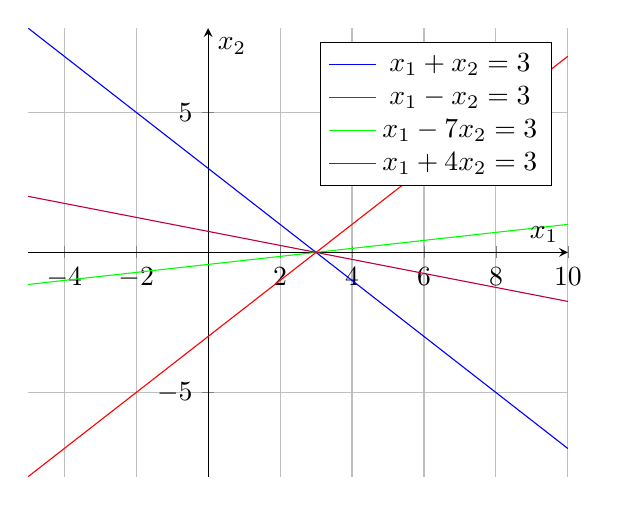
\begin{tikzpicture}
		\begin{axis}[
				axis lines = middle,
				xlabel = $x_1$,
				ylabel = $x_2$,
				grid = both,
				legend pos = north east
			]
			\addplot[
				domain=-5:10,
				samples=20,
				color=blue
			]
			{3-x};
			\addlegendentry{$x_1 + x_2 = 3$}
			\addplot[
				domain=-5:10,
				samples=20,
				color=red
			]
			{x-3};
			\addlegendentry{$x_1 - x_2 = 3$}
			\addplot[
				domain=-5:10,
				samples=20,
				color=green
			]
			{(x/7)-(3/7)};
			\addlegendentry{$x_1 - 7x_2 = 3$}
			\addplot[
				domain=-5:10,
				samples=20,
				color=purple
			]
			{(3/4)-(x/4)};
			\addlegendentry{$x_1 + 4x_2 = 3$}


		\end{axis}
	\end{tikzpicture}
	\caption{Plot of $x_1 + x_2 = 3$, $x_1 - x_2 = 3$, $x_1 - 7x_2 = 3$, and $x_1 + 4x_2 = 3$}
	\label{fig:plot5}
\end{figure}

\subsubsection*{B}

Unique solution since there exists a common intersection point of the lines.

\subsubsection*{C}

\[
	\begin{bmatrix}
		1 & 1  & 3 \\
		1 & -1 & 3 \\
		1 & -7 & 3 \\
		1 & 4  & 3
	\end{bmatrix}
	\xrightarrow{R_2 = R_2 - R_1, R_3 = R_3 - R_1, R_4 = R_4 - R_1}
	\begin{bmatrix}
		1 & 1  & 3 \\
		0 & -2 & 0 \\
		0 & -8 & 0 \\
		0 & 3  & 0
	\end{bmatrix}
	\xrightarrow{R_4=2R_4}
	\begin{bmatrix}
		1 & 1  & 3 \\
		0 & -2 & 0 \\
		0 & -8 & 0 \\
		0 & 6  & 0
	\end{bmatrix}
\]
\[
	\xrightarrow{R_4=R_4+3R_3, R_3=R_3-4R_2}
	\begin{bmatrix}
		1 & 1  & 3 \\
		0 & -2 & 0 \\
		0 & 0  & 0 \\
		0 & 0  & 0
	\end{bmatrix}
	\xrightarrow{R_2=-frac{1}{2}R_2}
	\begin{bmatrix}
		1 & 1 & 3 \\
		0 & 1 & 0 \\
		0 & 0 & 0 \\
		0 & 0 & 0
	\end{bmatrix}
	\xrightarrow{R_1=R_1-R_2}
	\begin{bmatrix}
		1 & 0 & 3 \\
		0 & 1 & 0 \\
		0 & 0 & 0 \\
		0 & 0 & 0
	\end{bmatrix}
\]
\subsubsection*{D}


\begin{verbatim}
    A = [1,1;1,-1;1,3;1,4];
    disp(rref(A))
\end{verbatim}

\color{lightgray}
\begin{verbatim}
         1     0
         0     1
         0     0
         0     0
\end{verbatim}
\color{black}


\subsubsection*{E}

\begin{verbatim}
    A = [1,1,3;1,-1,3;1,-7,3;1,4,3];
    disp(rref(A))
\end{verbatim}

\color{lightgray}
\begin{verbatim}
         1     0     3
         0     1     0
         0     0     0
         0     0     0
    
\end{verbatim}
\color{black}

\subsubsection*{F}

\[
	\begin{bmatrix}
		\tikz[baseline=(char.base)] \node[draw,circle,inner sep=2pt] (char) {1}; & 0                                                                        & 3 \\
		0                                                                        & \tikz[baseline=(char.base)] \node[draw,circle,inner sep=2pt] (char) {1}; & 0 \\
		0                                                                        & 0                                                                        & 0 \\
		0                                                                        & 0                                                                        & 0
	\end{bmatrix}
\]

Column 1: Pivot
Column 2: Pivot

\subsubsection*{G}

Yes, the SLE is indeed consistent and unique as predicted. By expanding the augmented matrix back to two equations we are left with $x_1 = 3, x_2 = 0$, which is indeed the same point shown in Fig.\ref{fig:plot5}.

\subsection*{System 6}

\subsubsection*{A}

-

\subsubsection*{B}

Since there are 3 equations in 5 unknowns, if the system is consistent it must have infinitely many solutions (with two free variables).

\subsubsection*{C}

\[
	\begin{bmatrix}
		1  & 1 & 1  & 1  & 1 & 4 \\
		-1 & 1 & -1 & 1  & 1 & 2 \\
		2  & 2 & 0  & -1 & 5 & 4
	\end{bmatrix}
	\xrightarrow{R_2 = R_2 + R_1,\quad R_3 = R_3 - 2R_1}
	\begin{bmatrix}
		1 & 1 & 1 & 1 & 1 & 4  \\
		0 & 2 & 0 & 2 & 2 & 6  \\
		0 & 0 & -2 & -3 & 3 & -4
	\end{bmatrix}
\]
\[
	\xrightarrow{R_2 = \frac{1}{2}R_2,\quad R_3 = -\frac{1}{2}R_3}
	\begin{bmatrix}
		1 & 1 & 1 & 1 & 1 & 4 \\
		0 & 1 & 0 & 1 & 1 & 3 \\
		0 & 0 & 1 & \frac{3}{2} & -\frac{3}{2} & 2
	\end{bmatrix}
\]
\[
	\xrightarrow{R_1 = R_1 - R_2}
	\begin{bmatrix}
		1 & 0 & 1 & 0 & 0 & 1 \\
		0 & 1 & 0 & 1 & 1 & 3 \\
		0 & 0 & 1 & \frac{3}{2} & -\frac{3}{2} & 2
	\end{bmatrix}
\]
\[
	\xrightarrow{R_1 = R_1 - R_3}
	\begin{bmatrix}
		1 & 0 & 0 & -\frac{3}{2} & \frac{3}{2} & -1 \\
		0 & 1 & 0 & 1 & 1 & 3 \\
		0 & 0 & 1 & \frac{3}{2} & -\frac{3}{2} & 2
	\end{bmatrix}
\]



\end{document}



